\chapter{Visualização de dados de plataformas de participação}
\section{Pol.is}

Pol.is é uma das referências deste trabalho e foi utilizado como uma das referências também de Software Livre para a construção do Empurrando Juntos por abordar as dimensões de governança digital, inclusão e manipulação. É uma plataforma que ajuda as organizações a se entenderem visualizando o que seus membros pensam \cite{poppi2017}. Para que tenham uma visão clara de todos os pontos de vista para ajudar a levar a conversa adiante \footnote{https://pol.is/home}. A inteligência do Pol.is foi utilizada nas primeiras versões do EJ.

Os criadores do Pol.is apontam a ineficiência na comunicação de grandes grupos de pessoas sobre determinados tópicos como o problema motivador para a criação da plataforma. Então, buscaram combinar técnicas de aprendizado de máquina e visualização interativa de dados em tempo real para Web. Afirma que o visual é voltado para o usuário, de forma simples e limpa, buscando estimular conversas e engajar participantes \footnote{https://www.geekwire.com/2014/startup-spotlight-polis/}.

%Ser a primeira empresa a combinar o aprendizado de máquina online (redes neurais..) com visualização interativa de dados em um aplicativo de Web em tempo real.

%Para os criadores do Pol.is, o problema era simples: a ineficiência de  grandes grupos de pessoas tentando se comunicar efetivamente sobre um determinado tópico on-line. E por isso desenvolveram uma maneira de combinar dados de pesquisa de centenas de pessoas com aprendizado de máquina e visualização interativa de dados. O resultado final é uma maneira simples e limpa para qualquer um, enquanto permite que os usuários estimulem conversas com base em todas as informações. \footnote{https://www.geekwire.com/2014/startup-spotlight-polis/}

\subsection{Evolução da visualização do Pol.is}

O objetivo dos criados do Pol.is sempre foi mostrar os grupos de opinião. E no processo de concepção dessa forma de visualização, no início queriam mostrar a “distância” entre os participantes com base em padrões de votação semelhantes e diferentes na conversa como elos, e esse agrupamento emergiria naturalmente disso, entretanto não foi isso que aconteceu. A primeira tentativa foi a visualização por meio de rede de grafos na Fig. \ref{fig01}, entretanto perceberam que tinha muitas informações à mostra, e decidiram não mostrar algumas informações utilizando a matemática. \footnote{https://blog.pol.is/the-evolution-of-the-pol-is-user-interface-9b7dccf54b2f}


\begin{figure}[h]
	\centering
	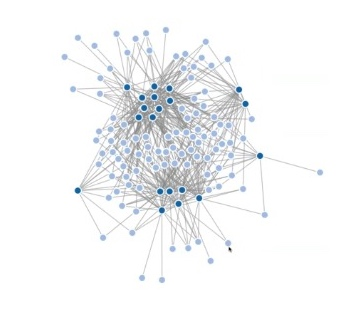
\includegraphics[keepaspectratio=true,scale=0.4]{figuras/evolucao-polis-1.png}
	\caption{Análise de grafos do Pol.is}
	Fonte: \url{https://blog.pol.is/the-evolution-of-the-pol-is-user-interface-9b7dccf54b2f}
	\label{fig01}
\end{figure}

A utilização de Análise de Componentes Principais (ou PCA em inglês), o que hoje é cerne do Pol.is mostra os dois primeiros principais componentes Fig. \ref{fig02} nos eixos x e y. Ocorre a perda de alguns dados na compactação para duas dimensões, mas preserva as maiores diferenças de opinião. 

Na Fig. \ref{fig02} é possível observar que cada participante é mostrado como um ponto preto e os vetores do PCA são expostos na visualização. Clicar nos círculos nos eixos traria os comentários associados àquele vetor - pessoas mais à esquerda, por exemplo, teriam maior probabilidade de concordar com alguma coleção de comentários.


\begin{figure}[h]
	\centering
	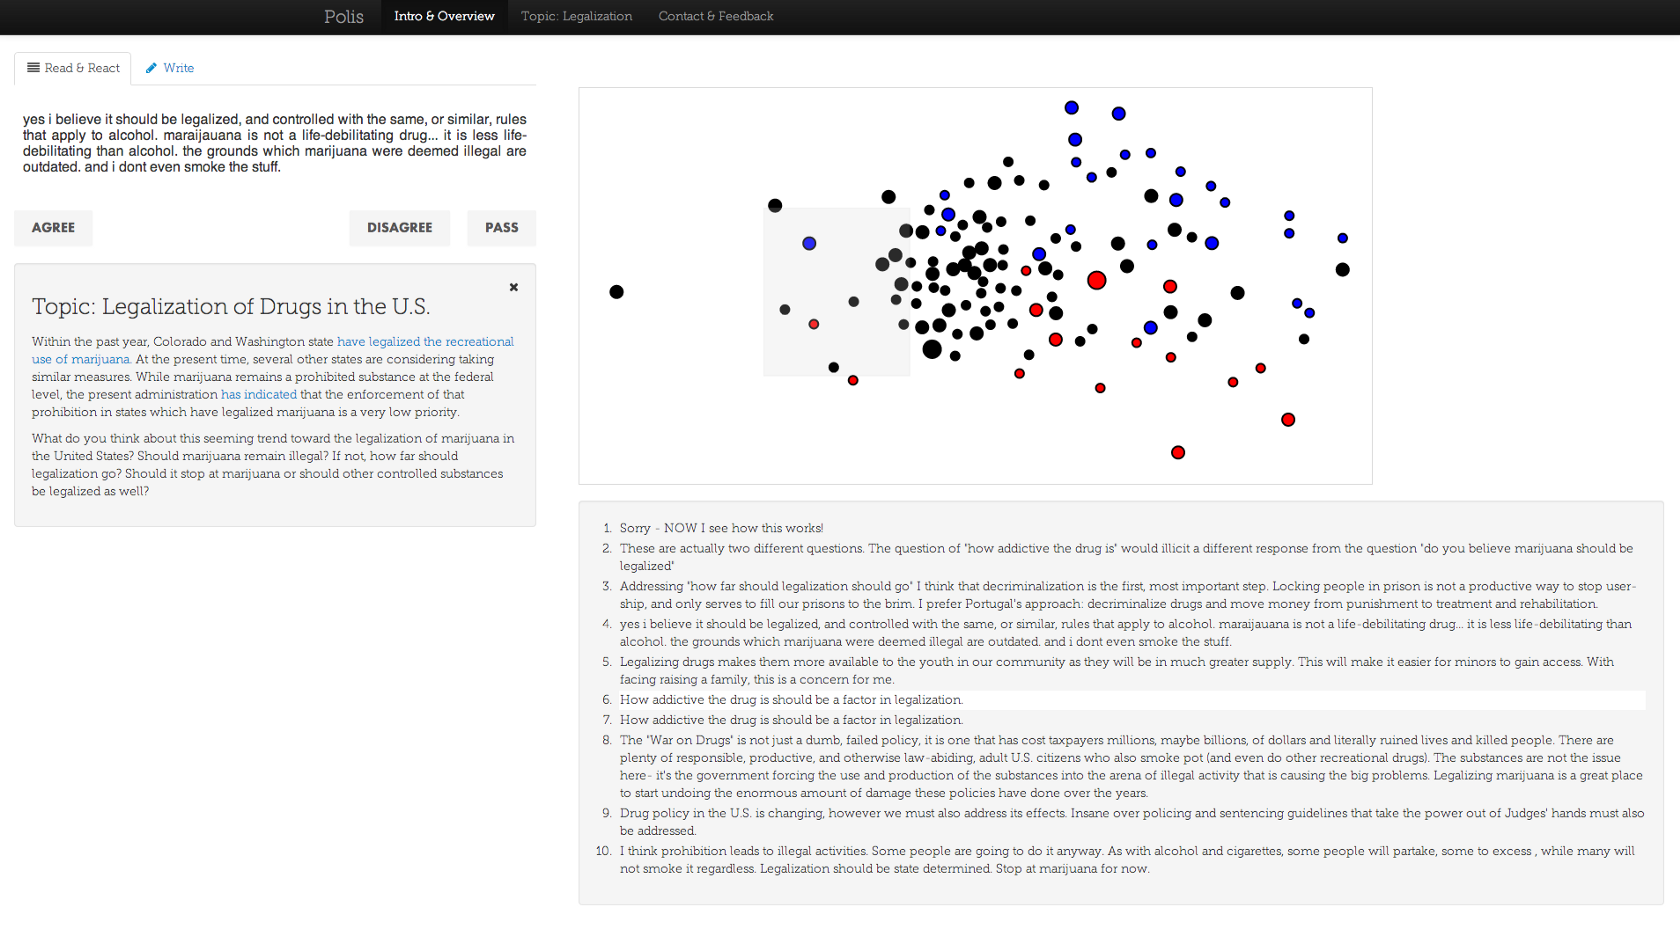
\includegraphics[keepaspectratio=true,scale=0.2]{figuras/evolucao-polis-2.png}
	\caption{Participantes e vetores do PCA do Pol.is}
	Fonte: \url{https://blog.pol.is/the-evolution-of-the-pol-is-user-interface-9b7dccf54b2f}
	\label{fig02}
\end{figure}


Para primeiro protótipo, Pol.is utilizou \textit{k-means} aos pontos e eliminou os pontos que tinham menos de um certo número de votos (eles tendiam a se agrupar no centro). Isso melhorou a sensação e começou a transmitir a ideia principal - há grupos de participantes que votaram de maneira semelhante e são um grupo porque compartilham um certo número de perspectivas, não apenas uma.

Dividiu os usuários em forma de seta, dimensionado proporcionalmente e um marcador no mapa, círculo azul, para enfatizar o aspecto espacial. Seguido da tarefa de criar uma correlação mais forte entre o comentário selecionado e o estado da visualização.

A suposição levantada pelos criados sobre o anonimato era muito restritiva. E colocar as pessoas na visualização resolveria todos os tipos de problemas, inclusive tornando a visualização muito mais concreta. O resultado deste trabalho pode ser visto na Fig \ref{fig03}. este foi o resultado 


\begin{figure}[h]
	\centering
	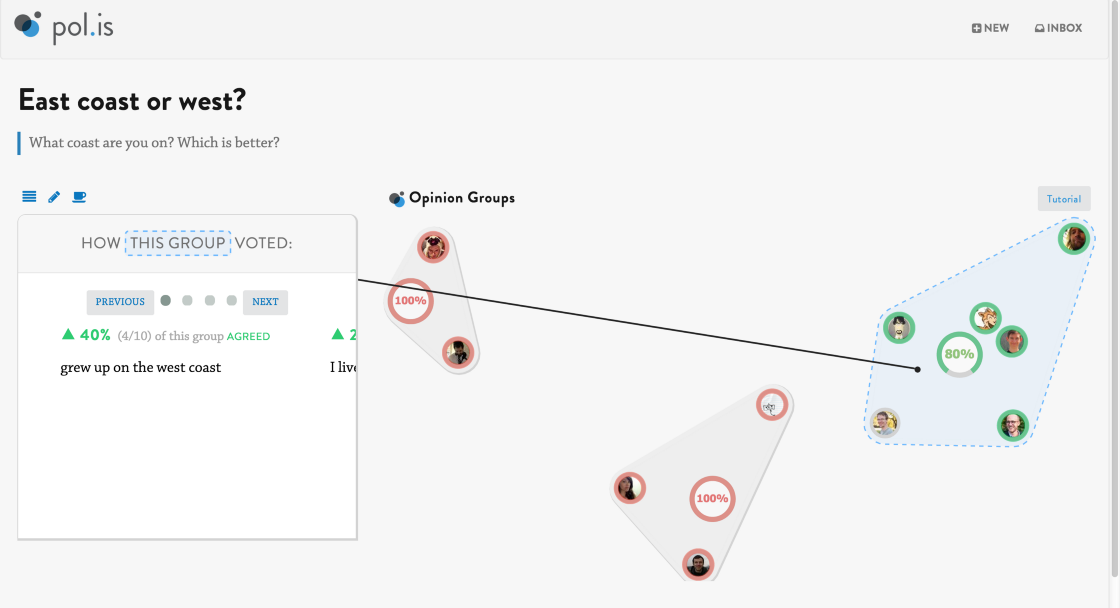
\includegraphics[keepaspectratio=true,scale=0.3]{figuras/evolucao-polis-3.png}
	\caption{Plataforma do Pol.is}
	Fonte: \url{https://blog.pol.is/the-evolution-of-the-pol-is-user-interface-9b7dccf54b2f}
	\label{fig03}
\end{figure}



\section{ConsiderIt}

ConsiderIt foi criado na Universidade de Washington, como parte da pesquisa de doutorado financiada pela National Science Foundation, com o objetivo de criar um método pelo qual grandes grupos de pessoas pudessem deliberar juntos e encontrar um terreno comum, mesmo em tópicos controversos.
\footnote{https://consider.it/tour?feature=moderation\#research}

A plataforma ConsiderIt pode ajudar a construir a confiança do público por meio de interfaces que encorajam as pessoas a considerar questões e refletir sobre as diversas perspectivas, enquanto é aprimorada a capacidade coletiva de tomar ações mais eficazes como reforma financeira e mudança climática \cite{bennett2012}.

ConsiderIt foi construído a partir do básico da deliberação pessoal para promover uma deliberação pública mais eficaz. É focado em fazer as pessoas pensarem sobre as compensações de uma ação proposta, como uma medida em uma eleição, convidando-os a criar uma lista de prós e contras como mostra a Fig \ref{fig04}. Em vez de apenas ter a opção binária de concorda ou não, existe a possibilidade de proporcionalidade de opinião, e a criação das listas com prós e contras. 

\begin{figure}[h]
	\centering
	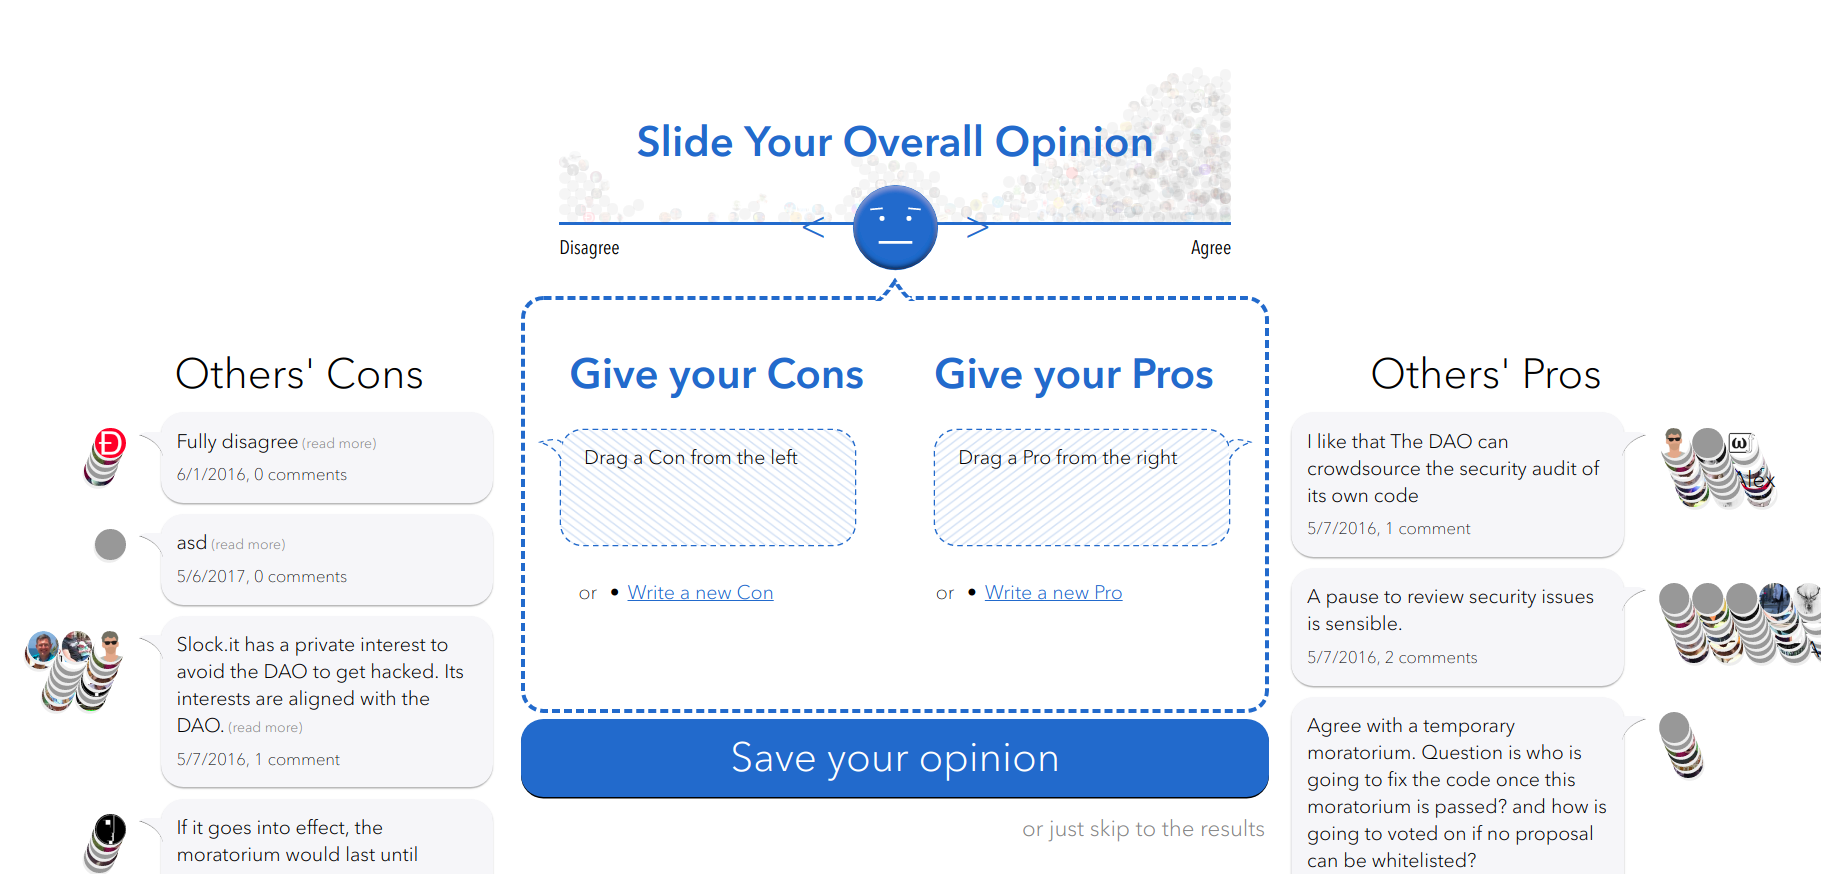
\includegraphics[keepaspectratio=true,scale=0.25]{figuras/teste-considerit.png}
	\caption{ConsiderIt}
	Fonte: \url{https://consider.it/examples}
	\label{fig04}
\end{figure}


ConsiderIt reaproveita essas deliberações pessoais para oferecer um guia em evolução para o pensamento público e apresenta as considerações mais notáveis pró e contra baseadas na frequência com que são incluídas e se são incluídas por pessoas com diferentes posições sobre o assunto. Também permite aprofundar os pontos relevantes para diferentes segmentos da população, podendo assim gerar \textit{insights} sobre as considerações de pessoas com diferentes perspectivas, podendo ajudar os usuários a identificar áreas comuns inesperadas. 

Também contribui com uma métrica de classificação de pró/contra feita para destacar pontos que ressoam com um público diverso, para promover pontos persuasivos e, ao mesmo tempo, incentivar uma diversidade de pontos de vista e, com sorte, resistir à manipulação estratégica.


\section{PolitEcho}

PolitEcho mostra o enviesamento político de amigos do Facebook e \textit{feed} de notícias de um usuário. É uma extensão do Google Chrome que conecta com o Facebook e atribui a cada amigo uma pontuação baseada em uma previsão de tendências políticas e exibe um gráfico da lista de amigos. Em seguida, calcula o viés político no conteúdo do feed de notícias e compara-o com o viés da lista de amigos para destacar possíveis diferenças entre os dois. As cores azul e vermelho representam viés liberal e conservador respectivamente como pode ser visto na Fig \ref{fig05}.


\begin{figure}[h]
	\centering
	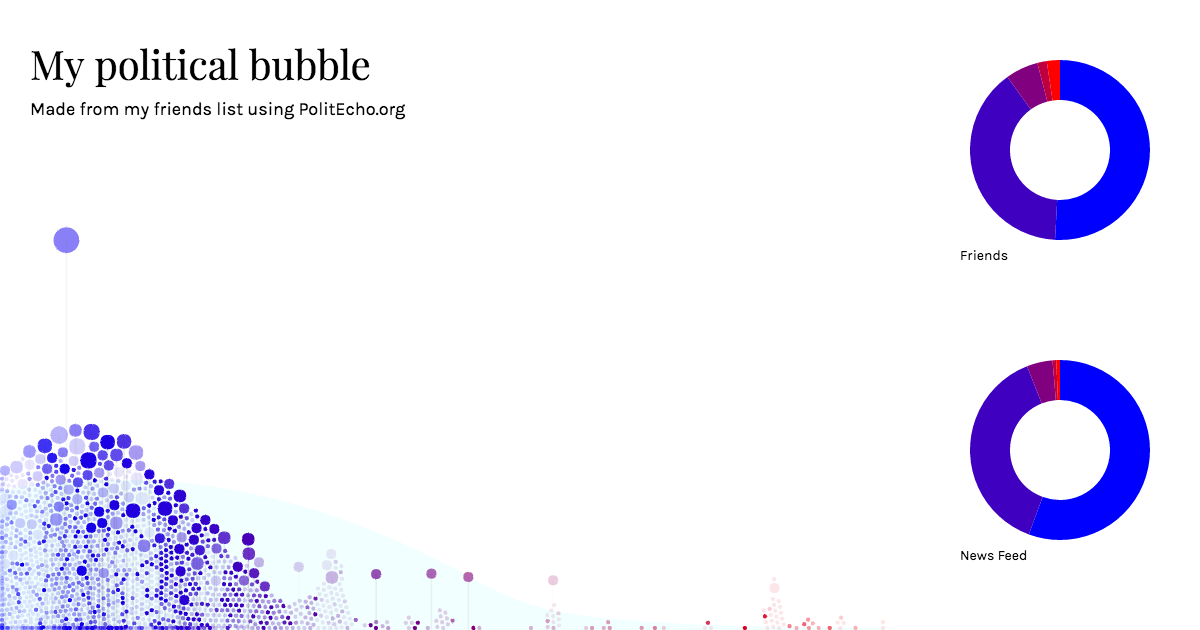
\includegraphics[keepaspectratio=true,scale=0.3]{figuras/politecho.png}
	\caption{PolitEcho}
	Fonte: \url{https://politecho.org/}
	\label{fig05}
\end{figure}


As avaliações políticas dos amigos são baseadas nas páginas políticas do Facebook que eles gostam. É comparada as páginas que os amigos gostaram em um banco de dados de páginas do Facebook que foram classificadas por seu viés liberal/conservador e, é computado uma pontuação com base em quaisquer correspondências. \footnote{https://politecho.org/}